\documentclass[12pt]{article}

\usepackage{amsmath}
\usepackage{array}
\usepackage{enumitem}
\usepackage{float}
\usepackage[margin=1in]{geometry}
\usepackage{graphicx}
\usepackage{hhline}
\usepackage{hyperref}
\hypersetup{colorlinks=true, citecolor=magenta, linkcolor=blue, urlcolor=cyan}
\usepackage{multirow}
\usepackage[all]{nowidow} 
\usepackage{parskip}
\usepackage{pdfpages}
\usepackage{subcaption}
\usepackage{titlesec}
\titleformat*{\section}{\large\bfseries}
\titleformat*{\subsection}{\normalsize\bfseries}
\usepackage{xcolor}

\usepackage[abs]{overpic}
\usepackage{pict2e}

\usepackage{tikz}
\usetikzlibrary{plotmarks}
\usetikzlibrary{shapes.geometric, arrows}
\tikzstyle{box} = [rectangle, rounded corners, minimum width=1.2cm, minimum height=1.2cm, draw=black, line width=0.4mm]
\tikzstyle{arrow} = [thick, ->, >=stealth]



\begin{document}
	
\section*{SIR Model with Optimal Control Example}

By: Lindsey Fox at Eckerd College \\

In a mathematical model, there may be one or more parameters that can be controlled in some manner to affect the dynamics of the system. Optimal Control Theory is a branch of mathematical optimization that finds the best way to control the parameters to achieve a certain goal. The following introduction to Optimal Control Theory follows from the text by Lenhart and Workman \cite{OCBook} and will be applied to the SIR framework, as an example.

For our purposes we will define $u(t)$ as the model parameter(s) we wish to control and $x(t, u)$ to be the state variable(s) we want to drive to a certain result. The state represents the underlying dynamical system constrained by the system of equations $g(t, u, x)$ in \eqref{eqn:constraint}. Ultimately, the goal in \eqref{eqn:goal} is to find the function $u^*(t)$, and the corresponding state $x^*(t, u^*)$, that maximizes the objective functional $J(u)$ at each point in time over the time interval $[t_0, t_1]$. The following framework can be easily adapted to a minimization problem as is shown in the SIR example later.

% eqn:constraint
\begin{equation} \label{eqn:constraint}
	\begin{aligned}
		\frac{dx}{dt} &= g(t, u, x) \\[5pt] 
		x(0) &= x_0
	\end{aligned}
\end{equation}

% eqn:goal
\begin{equation} \label{eqn:goal}
	u^*(t) = \max\limits_{u} J(u) = \max\limits_{u} \int_{t_0}^{t_1} f(t, u, x) dt
\end{equation}

To find $u^*(t)$, we form the Hamiltonian in \eqref{eqn:ham} to append the constraint in \eqref{eqn:constraint} to the goal in \eqref{eqn:goal}. This is similar to a Lagrangian expression in a static optimization problem. The main difference is that the equivalent of the Lagrange multiplier, $\lambda(t)$, referred to as the adjoint equation here, is a function of time rather than a constant.

% eqn:ham
\begin{equation} \label{eqn:ham}
	H = f + \lambda g
\end{equation}

Pontryagin's Maximum Principle states that in order for $u^*(t)$ to exist, there are two necessary conditions that must be satisfied. The first order condition, given in \eqref{eqn:1st}, is that the Hamiltonian is maximized at $u^*(t)$, meaning that the derivative of $H$ with respect to $u$ evaluated at $u^*$ is zero. The second order condition, given in \eqref{eqn:2nd}, is that the Hamiltonian must have the correct convexity in order for $u^*(t)$ to be a maximum.

% eqn:1st
\begin{equation} \label{eqn:1st}
	\frac{\partial H}{\partial u}\Big|_{u^*} = \Big[ \frac{\partial f}{\partial u} + \lambda \frac{\partial g}{\partial u} \Big] \Big|_{u^*} = 0 
\end{equation}

% eqn:2nd
\begin{equation} \label{eqn:2nd}
	\frac{\partial^2 H}{\partial u^2} \Big|_{u^*} \leq 0
\end{equation}

Solving \eqref{eqn:1st} for $u^*(t)$ will give an expression for $u^*(t)$ as a function of $\lambda$. In order to have an expression for $u^*(t)$ only as a function of time we must solve the adjoint equation in \eqref{eqn:adj}.

% eqn:adj
\begin{equation} \label{eqn:adj}
	\begin{aligned}
		\frac{d\lambda}{dt} &= -\frac{\partial H}{\partial x} = - \Big(\frac{\partial f}{\partial x} + \lambda \frac{\partial g}{\partial x}\Big) \\[5pt]
		\lambda(t_1) &= 0
	\end{aligned}
\end{equation}

In some scenarios, like the SIR example below, we may require that the control is bounded, adding an additional constraint on the system. In this case, we require \eqref{eqn:uset} to hold.

% eqn:uset
\begin{equation} \label{eqn:uset}
	u(t) \in \big\{ L^{\infty}[t_0, t_1] \,\, \big| \,\, u_{\min} \leq u(t) \leq u_{\max} \big\}
\end{equation}

Now consider the SIR model shown in Figure \ref{fig:SIRv}, where $S(t)$ represents the number of susceptible individuals at time $t$, $I(t)$ represents the number of infectious individuals at time $t$, and $R(t)$ represents the number of removed individuals at time $t$. The parameters of the model are $\beta$, the rate of infection, and $\gamma$, the rate of recovery. 

The control is the vaccination rate $v(t)$. Vaccination moves susceptible individuals directly into the removed compartment. The state variables are $x(t) = [S(t) \,\, I(t) \,\, R(t)]^T$ and are constrained by $g(t) = [\frac{dS}{dt} \,\, \frac{dI}{dt} \,\, \frac{dR}{dt}]^T$ in \eqref{eqn:SIRv}. We also require that $0 \leq v(t) \leq v_{\max}$ because a vaccination rate cannot be negative and there is an upper limit to the number of individuals that can be vaccinated in a single day.

\begin{figure}[H] 
	\begin{center}
		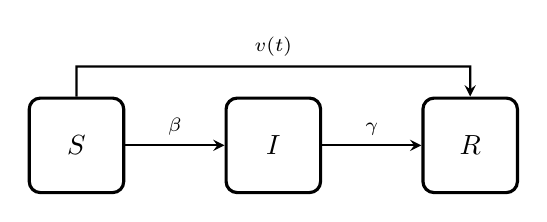
\begin{tikzpicture}[node distance=2.5cm]
			\node (S) [box] {$S$};
			\node (I) [box, right of=S] {$I$};
			\node (R) [box, right of=I] {$R$};
			\draw [arrow] (S) -- node[anchor=south] {$\scriptstyle \beta $} (I);
			\draw [arrow] (I) -- node[anchor=south] {$\scriptstyle \gamma$} (R);
			\draw [arrow] (S) to (0,1) -- node[anchor=south] {$\scriptstyle v(t) $} (5,1) to (R);
		\end{tikzpicture}
		\caption[SIR Model with Vaccination Schematic] {Schematic representation of the SIR model. $S(t)$, $I(t)$, and $R(t)$ are the total number of susceptible, infected, and removed individuals, respectively, at a given time $t$. Model parameters include the infection rate $\beta$, recovery rate $\gamma$, and vaccination rate $v(t)$.}
		\label{fig:SIRv}
	\end{center}
\end{figure}

\vspace{-20pt}

% eqn:SIRv
\begin{equation} \label{eqn:SIRv}
	\begin{aligned} 
		\frac{dS}{dt} &= -\beta I S - v(t)S \\[5pt]
		\frac{dI}{dt} &= \beta I S - \gamma I \\[5pt]
		\frac{dR}{dt} &= \gamma I + v(t) S
	\end{aligned}
\end{equation}

In an example scenario, the goal is to find a function, $v^*(t)$, such that the cost of cases and the cost of vaccination are both minimized, where the integral of $\beta IS$ over the time period $[0, T]$ is the total number of cases, $C_1$ is the relative cost per case, $C_2$ is the relative cost per vaccination, and $\epsilon$ is an additional nonlinear relative cost of vaccination. This goal is described in \eqref{eqn:goalv}. 

% eqn:goalv
\begin{equation} \label{eqn:goalv}
	v^*(t) = \min\limits_{0 \leq v \leq v_{\max}} J(v) = \min\limits_{0 \leq v \leq v_{\max}} \int_0^T (C_1\beta IS + C_2vS + \epsilon v^2) dt 
\end{equation} 

It is important to note that since $0 \leq v(t) \leq v_{\max} \leq 1$, the nonlinear term $v^2$ will be very small. This represents a small additional cost for increasing the vaccination rate. For most vaccination programs, most costs come up front in the development of the vaccine itself and the distribution procedure. Once those are implemented, vaccinating additional individuals is a relatively small increase in cost. 

The Hamiltonian for this optimality system is given in \eqref{eqn:hamv}. The first order condition is given in \eqref{eqn:1stv}. The optimal vaccination rate $v^*(t)$ is given in \eqref{eqn:vstar}, ensuring that the vaccination rate remains bounded. The second order condition is given in \eqref{eqn:2ndv}, ensuring that $v^*(t)$ is indeed a minimum at each time point since $\epsilon$ is a positive cost. The adjoint equations are given in \eqref{eqn:adjv}, where the adjoints are $\lambda = [\lambda_S \,\, \lambda_I \,\, \lambda_R]$.

% eqn:hamv
\begin{equation} \label{eqn:hamv}
	\begin{aligned}
		H &= f + \lambda g = f + \lambda_S \cdot \frac{dS}{dt} + \lambda_I \cdot \frac{dI}{dt} + \lambda_R \cdot \frac{dR}{dt} \\[5pt]
		&= C_1\beta IS + C_2v + \epsilon v^2 + \lambda_S (-\beta IS - vS) + \lambda_I (\beta IS - \gamma I) + \lambda_R (\gamma I + vS)
	\end{aligned}
\end{equation}

% eqn:1stv
\begin{equation} \label{eqn:1stv}
	\frac{\partial H}{\partial v} \Big|_{v^*} = C_2 + 2\epsilon v^* + \lambda_S (-S) + \lambda_R (S) = 0
\end{equation}

% eqn:vstar
\begin{equation} \label{eqn:vstar}
	v^*(t) = \min \Bigg\{ v_{\max}, \max \Big\{ 0, \frac{-C_2 + \lambda_SS - \lambda_RS}{2\epsilon} \Big\} \Bigg\}
\end{equation}

% eqn:2ndv
\begin{equation} \label{eqn:2ndv}
	\frac{\partial^2 H}{\partial v^2} \Big|_{v^*} = 2\epsilon \geq 0
\end{equation}

% eqn:adjv
\begin{equation} \label{eqn:adjv}
	\begin{aligned}
		\frac{d\lambda_S}{dt} &= -\frac{\partial H}{\partial S} \\[5pt]
		&= -\big( C_1\beta I + \lambda_S (-\beta I - v) + \lambda_I (\beta I) + \lambda_R (v) \big) \\[15pt]
		\frac{d\lambda_I}{dt} &= -\frac{\partial H}{\partial I} \\[5pt]
		&= -\big( C_1\beta S + \lambda_S (-\beta S) + \lambda_I (\beta S - \gamma) + \lambda_R (\gamma) \big) \\[15pt]
		\frac{d\lambda_R}{dt} &= -\frac{\partial H}{\partial R} \\[5pt]
		&= -\big( 0 \big) \\[15pt]
		\lambda_i(T) &= 0, \quad i = S, I, R
	\end{aligned}
\end{equation}

\pagebreak

The solution of an optimality system is simulated using a numerical method called the Forward-Backwards Sweep. A pseudo-code for the algorithm is given below. 

{\texttt{
		\begin{enumerate}
			\item Make an initial guess for $u^*$.
			\item Solve for $x$ forward in time using the initial condition $x(t_0) = x_0$.
			\item Solve for $\lambda$ backwards in time using the final time condition $\lambda(t_1) = 0$.
			\item Update $u^*$ based on the characterization by $x$ and $\lambda$. 
			$$ u^*_{\text{new}} = \frac{u^*_{\text{char}} + u^*_{\text{old}}}{2} $$
			\item Check convergence for some accepted tolerance $\delta$.
			$$ \frac{|u^*_{\text{new}} - u^*_{\text{old}}|}{|u^*_{\text{new}}|} \leq \delta $$
			\item Return to step 2 if the convergence criteria is not satisfied.
\end{enumerate}}}
\vspace{25pt}

Figure \ref{fig:SIRr} shows a simulation of the SIR model without vaccination. Compare this with Figure \ref{fig:SIRvr}, which shows the same simulation of the SIR model but with the optimal vaccination $v^*(t)$ as determined by the optimality system. Figure \ref{fig:SIRr} was generated from the R code \texttt{SIR.r} and Figure \ref{fig:SIRvr} was generated from the R code \texttt{SIR\_OC.r}. Similar figures (\ref{fig:SIRm} and \ref{fig:SIRvm}) can be produced by the MATLAB files \texttt{SIR.m} and \texttt{SIR\_OC.m}. 

% fig:SIRr
\begin{figure}[H] 
	\centering
	\includegraphics[scale=0.5]{SIRr.png}
	\caption{Simulation of the SIR model over 150 days without vaccination. Initial conditions are $S(0) = 9,999$, $I(0) = 1$, and $R(0) = 0$ individuals. Model parameters are $\beta = 0.00009$ per individual per day and $\gamma = 0.05$ per day. There is a total of 9,999 cases. This figure was generated by the R code \texttt{SIR.r}.}
	\label{fig:SIRr}
\end{figure}

% fig:SIRvr
\begin{figure}[H] 
	\centering
	\includegraphics[scale=0.5]{SIRvr.png}
	\caption{(a) Simulation of the SIR model over 150 days with the (b) optimal vaccination rate $v^*(t)$. Initial conditions are $S(0) = 9,999$, $I(0) = 1$, and $R(0) = 0$ individuals. Model parameters are $\beta = 0.00009$ per individual per day and $\gamma = 0.05$ per day. Cost parameters are $C_1 = 1$, $C_2 = 0.1$, and $\epsilon = 100$. The maximum vaccination rate is $v_{\max} = 0.05$. There is a total of 4,902 cases. This figure was generated by the R code \texttt{SIR\_OC.r}.}
	\label{fig:SIRvr}
\end{figure}

In Figure \ref{fig:SIRr}, we see that the epidemic peaks around day 15 with over $7,800$ cases, the epidemic dies out around day 100, and the total number of cases is $9,999$, meaning everyone in the population got sick. In Figure \ref{fig:SIRvr}, we see that the epidemic peaks a little later around day 20 with over $3,300$ cases, the epidemic also dies out around day 100, and the total number of cases is $4,902$, which is less than half of the total number of cases in the simulation without vaccination. The optimal vaccination rate remains at the maximum vaccination rate of $5\%$ per day until about day 30, when the number of infectious individuals drops below $2,500$ individuals. After this point, the optimal vaccination rate decreases quickly to zero. The solution of the optimality system tells us that we vaccinate as many people as we can early in the epidemic, but when we have gone past the peak of the epidemic, we no longer need to vaccinate since the epidemic is now dying out. 

% fig:SIRm
\begin{figure}[H] 
	\centering
	\includegraphics[scale=0.25]{SIRm.png}
	\caption{Same as Figure \ref{fig:SIRr} but generated by the MATLAB code \texttt{SIR.m}.}
	\label{fig:SIRm}
\end{figure}

% fig:SIRvm
\begin{figure}[H] 
	\centering
	\includegraphics[scale=0.25]{SIRvm.png}
	\caption{Same as Figure \ref{fig:SIRvr} but generated by the MATLAB code \texttt{SIR\_OC.m}.}
	\label{fig:SIRvm}
\end{figure}

\bibliographystyle{plain}
\bibliography{references.bib}

\end{document}